Test Case~1a uses a set of five precomputed ground motion values to test the correct interpolation of the mean loss ratios of the vulnerability function at intermediate intensity measure levels. There is no uncertainty in the vulnerability function used for this case. The coefficient of variation of the loss ratio is zero at all intensity measure levels.

\begin{table}[htbp]

\centering
\begin{tabular}{ l c c l }

\hline
\rowcolor{anti-flashwhite}
\bf{GMF \#} & \bf{Site} & \bf{PGA (g)}\\
\hline
1 & 1 & 1.300 \\
2 & 1 & 0.044 \\
3 & 1 & 0.520 \\
4 & 1 & 1.000 \\
5 & 1 & 1.200 \\
\hline
\end{tabular}

\caption{Five precomputed ground motion fields at a single site}
\label{tab:gmfs-diff-l1-5}
\end{table}

Table~\ref{tab:gmfs-diff-l1-5} lists the five ground motion values used in this test case.

\begin{table}[htbp]

\centering
\begin{tabular}{ l c c c c c c c c c c c}

\hline
\rowcolor{anti-flashwhite}
\bf{PGA} & 0.05 & 0.20 & 0.40 & 0.60 & 0.80 & 1.00 & 1.20 & 1.40 & 1.60 & 1.80 & 2.00 \\
\hline
\bf{Mean LR} & 0.01 & 0.04 & 0.10 & 0.20 & 0.33 & 0.50 & 0.67 & 0.80 & 0.90 & 0.96 & 0.99 \\
\bf{CoV LR} & 0.0 & 0.0 & 0.0 & 0.0 & 0.0 & 0.0 & 0.0 & 0.0 & 0.0 & 0.0 & 0.0 \\
\hline
\end{tabular}

\caption{Vulnerability function with zero coefficients of variation}
\label{tab:vf-ln-tax1-zcov}
\end{table}

Table~\ref{tab:vf-ln-tax1-zcov} shows the mean loss ratios and corresponding coefficients of variation in the lognormal vulnerability function used in this test case. The vulnerability model is shown in Figure~\ref{fig:vf-ln-tax1-zcov}, where the dots represent the median loss ratios at a set of intensity levels.

\begin{figure}[htbp]
\centering
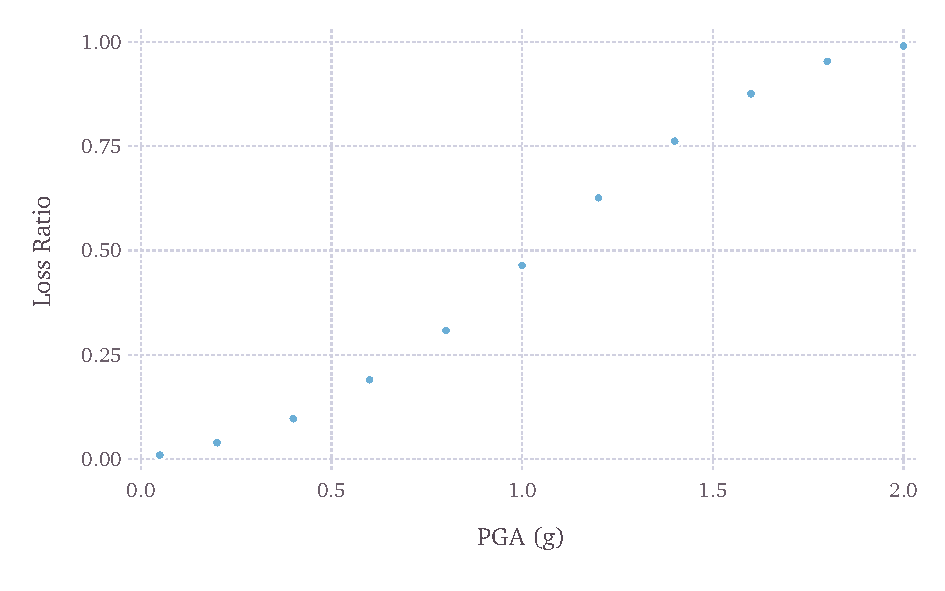
\includegraphics[width=12cm]{qareport/figures/fig-vf-ln-tax1-zcov}
\caption{Vulnerability model with zero coefficients of variation}
\label{fig:vf-ln-tax1-zcov}
\end{figure}

Since there is no variability in the loss ratio, calculation of the loss ratios is straightforward in this case. Since the coefficients of variation in the vulnerability function are all zero, the lognormal distribution devolves into the degenerate distribution. The ground motion values at the location of the single asset are $[1.3, 0.044, 0.52, 1.0, 1.2] g$. Consider the first value of $PGA = 1.3 g$. The vulnerability function for this case provides mean loss ratio values at intensity measure levels $1.2 g$ and $1.4 g$, but none at $1.3 g$. The mean loss ratios at $1.2 g$ and $1.4 g$ are $0.67$ and $0.80$ respectively.

The mean loss ratio at $1.3 g$ is obtained by interpolating between these two values. Linear interpolation gives a mean loss ratio of $0.735$ for $PGA = 1.3 g$.

Similar interpolation for the other ground motion values gives mean loss ratios of $0$, $0.16$, $0.5$, and $0.67$.

The mean loss ratio is simply obtained as the arithmetic mean of the five loss ratios as:

\begin{equation*}
\frac{0.735 + 0.0 + 0.16 + 0.50 + 0.67}{5} = 0.413
\end{equation*}

The standard deviation of the loss ratio is computed as:

\begin{multline*}
\sqrt{\frac{(0.735 - 0.413)^2 + (0.0 - 0.413)^2 + (0.16 - 0.413)^2 + (0.50 - 0.413)^2 + (0.67 - 0.413)^2}{5 - 1}} \\
= 0.320889
\end{multline*}

These numbers are multiplied by the asset value of $10,000$ to give the mean and standard deviation of loss for the scenario as $4,130$ and $3,208.89$ respectively.